\section{A Classical Slice That Looks Right}\label{sec:example}

\begin{figure}[t]
  \centering
  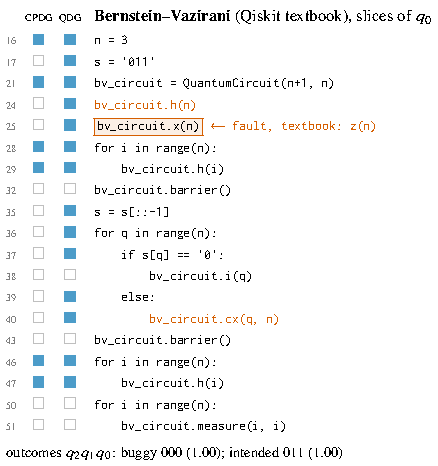
\includegraphics[width=\columnwidth]{figures/fig_bv.pdf}
  \caption{The Bernstein--Vazirani program of the Qiskit textbook~\cite{qiskittextbook}, with comments and blank lines
  omitted and the textbook's line numbers kept. Line~25 carries a seeded fault, \texttt{x(n)} where the textbook
  applies \texttt{z(n)}. The two columns mark the lines in the backward slice of $q_0$ under the classical PDG and
  under the QDG. The classical slice misses the orange lines, which can change $q_0$. Slices are computed statically
  by \tool{}, and outcomes and dependences by the study's code.}
  \label{fig:bv}
\end{figure}

This section shows, on a textbook program, how a slice computed the classical way can reproduce the output a
developer sees and still hide the fault, and why a check of measured outcomes cannot tell. It starts with the
quantum concepts the rest of the paper uses.

\paragraph*{Background}
A qubit's state is a superposition $\alpha\ket{0} + \beta\ket{1}$, and measuring it yields $0$ or $1$ with
probabilities $|\alpha|^2$ and $|\beta|^2$. The two states $\ket{+}$ and $\ket{-}$ give both outcomes equally often
and differ only in the sign of $\beta$, their phase, which no measurement in the computational basis can see. Gates are
reversible operations on qubits, such as the Hadamard gate H, which turns $\ket{0}$ into $\ket{+}$ and $\ket{+}$ back
into $\ket{0}$. A controlled gate such as the controlled-NOT (CNOT) applies an operation to its target depending on
its control, but it can also change the control. When the target is in $\ket{-}$, the CNOT leaves the target as it is
and flips the phase of its control instead, an effect called phase kickback. Two qubits are entangled when their
joint state cannot be written as a state of each qubit alone. A measurement writes a classical bit, which later gates
may read as a condition. Qiskit programs build circuits in Python, with loops, functions and conditions that compute
which gates act on which qubits.

\paragraph*{The program}
The Bernstein--Vazirani algorithm~\cite{bernstein1997qct} finds a hidden bit string $s$ with a single query to an
oracle. Fig.~\ref{fig:bv} shows the program of the Qiskit textbook~\cite{qiskittextbook}, with $s = 011$. It rests on
phase kickback. Lines~24 and~25 prepare the auxiliary qubit $q_3$ in $\ket{-}$, line~29 puts every data qubit in
$\ket{+}$, and for every bit of $s$ that is $1$, the CNOT of line~40 kicks a phase onto its data qubit, turning
$\ket{+}$ into $\ket{-}$. The Hadamard gates of line~47 turn these phases into the bits of $s$, so the program
returns~$011$. We seeded one fault, a one-token change on line~25 that applies X instead of Z. The auxiliary is
then left in $\ket{+}$, on which a CNOT changes nothing, and the program returns \numBvBuggyOut{} instead of
\numBvFixedOut{}.

\paragraph*{The slices}
The developer sees $q_0$ read $0$ where $s$ says $1$, and slices backward from $q_0$ to see which lines determine it.
A classical slicer reads \texttt{cx(q, n)}, which flips its target when its control is $1$, as the assignment
$q_n \leftarrow q_n \oplus q$, which reads $q$ and writes only the auxiliary. Its slice of $q_0$ keeps the Hadamard
gates of lines~\numBvCpdgLines{} and the lines that compute their qubits, lines \numBvCpdgClassical{}, as the left
column of Fig.~\ref{fig:bv} shows. The slice looks right. Its \numBvCpdgOps{} operations give $q_0$ the same state as
the faulty program, with fidelity \numBvCpdgFidelity{}, a similarity of quantum states that is $1$ exactly when they
are equal, so it gives the developer no reason to look at lines~\numBvMissedLines{}, where the fault is.

These lines can nonetheless change $q_0$. Restoring Z on line~25 turns $q_0$ from $\ket{0}$ into $\ket{1}$, two states
with fidelity \numBvFixFidelity{}, because the CNOT acts on its control as well as its target. A slice that lets
every gate write all its qubits, the QDG of Section~\ref{sec:core}, keeps lines~\numBvQdgLines{}, together with the
lines that compute them, among them the oracle's loop and condition on lines~35 to~39. Its slice contains the fault. The QPDG of Yu and Zhao keeps the same lines here, since its two extra operations, the Hadamard gate and the
CNOT of $q_1$, are later iterations of lines~29 and~40 that cannot change $q_0$, and Fig.~\ref{fig:ansatz} shows where
it costs more.

\paragraph*{Why the outcomes cannot tell}
Here the fault shows in the measured outcome of $q_0$. That is not always so. In a real bug from
Bugs4Q~\cite{zhao2023bugs4q}, posted on Stack Overflow, a two-qubit program meant to prepare
$(\ket{01}+\ket{10})/\sqrt{2}$ applies \texttt{h(0)}, \texttt{h(1)} and \texttt{cx(0,1)}, with \texttt{h(1)} where
\texttt{x(1)} was needed, and returns all four bit strings equally often. Each qubit alone reads $1$ with probability
\numMotPOne{}, in the buggy program and in the intended one alike, so the outcomes of either qubit cannot reveal the
failure, and only their joint outcomes do. The fault does change the state of $q_0$, which is a uniformly random bit in
the intended program and the pure $\ket{+}$ in the buggy one, two states with fidelity \numMotFidelity{}. Because the
CNOT writes its control, the QDG slice of $q_0$ contains the faulty \texttt{h(1)}, while the classical slice keeps only
\texttt{h(0)}.

Both lessons hold beyond these programs, as Section~\ref{sec:results} shows. Reading a gate as an assignment misses
influence that flows into a control qubit, and judging a slice by the outcomes of one qubit misses errors in phase and
in correlations. A slice must therefore be judged by the state of the qubits it is about, which is how
Section~\ref{sec:core} defines it.
